


In this section, we first provide a background of the
{\em Open Web Archive} Data Model in which we describe the data model
along with a sample depiction of a non-versioned article as
in the semantic layer.
Then we mention the different works related to ranking of archived documents,
ranking in knowledge graphs and
ranking documents in knowledge graphs.

\subsection{The \q{Open Web Archive} Data Model}
\label{subsec:semanticmodel}

\-\hspace{0.5cm}In our previous work\cite{fafalios2017SemLayer} we introduced an RDF/S data model to describe
the semantic information and metadata about the documents
of a web archive.
This model, which we call as {\em Open Web Archive} data model\footnote{Specification publicly
available at: \url{http://l3s.de/owa/}},
is depicted in Figure \ref{fig:owa}.
We re-use elements from many other existing data models
and define 2 new classes and 3 new properties.
An archived document is represented using the class {\tt owa:Archi\-ved\-Do\-cu\-ment}.
Further, the archived document may or may not be linked with some versions
(i.e., instances of {\tt owa:Ve\-rsio\-ned\-Do\-cu\-ment}).
Versions pages for billions of web sites can be
found on the Internet Archive.
In contrast, the New York Times corpus \cite{sandhaus2008new} that we
try applying our ranking models on does
not contain versions.

We associate an archived document
with three main elements:
i) metadata information, like format(mime type),
date of capture/publication, and document title,
ii) links to other documents (web pages), archived or not, and
iii) set of annotations.
Terms from the Dublin Core Metadata Initiative\footnote{\url{http://dublincore.org/}}
were used to describe some of the metadata.
Annotations were described by exploiting
the Open Annotation Data Model \cite{sanderson2013open}
and the Open Named Entity Extraction (NEE) Model \cite{fafalios2015ijait}. % \footnote{\url{http://www.ics.forth.gr/isl/oae/}}

The Open Annotation Data Model contains an RDF-based framework specification for creating associations (annotations)
between related resources, while the Open NEE Model is an extension
that allows describing the result of an entity extraction process.
An annotation has a {\em target}, which is an archived document in our case, and
a {\em body} which is a concept, entity or event
mentioned in the document.
An archived document can be directly related with an
entity, concept or event by exploiting the property \q{{\tt mentions}}
of schema.org\footnote{\url{http://schema.org/mentions}} for reducing the
number of derived triples.
A concept, entity or event can be associated with information like
its name, a confidence score, its position in the document, and a resource (URI).
The URI enables to retrieve additional information from the Linked Open Data (LOD)
cloud \cite{heath2011linked} (like properties, relations with other entities, etc.).

\begin{figure}[H]
\centering
\fbox{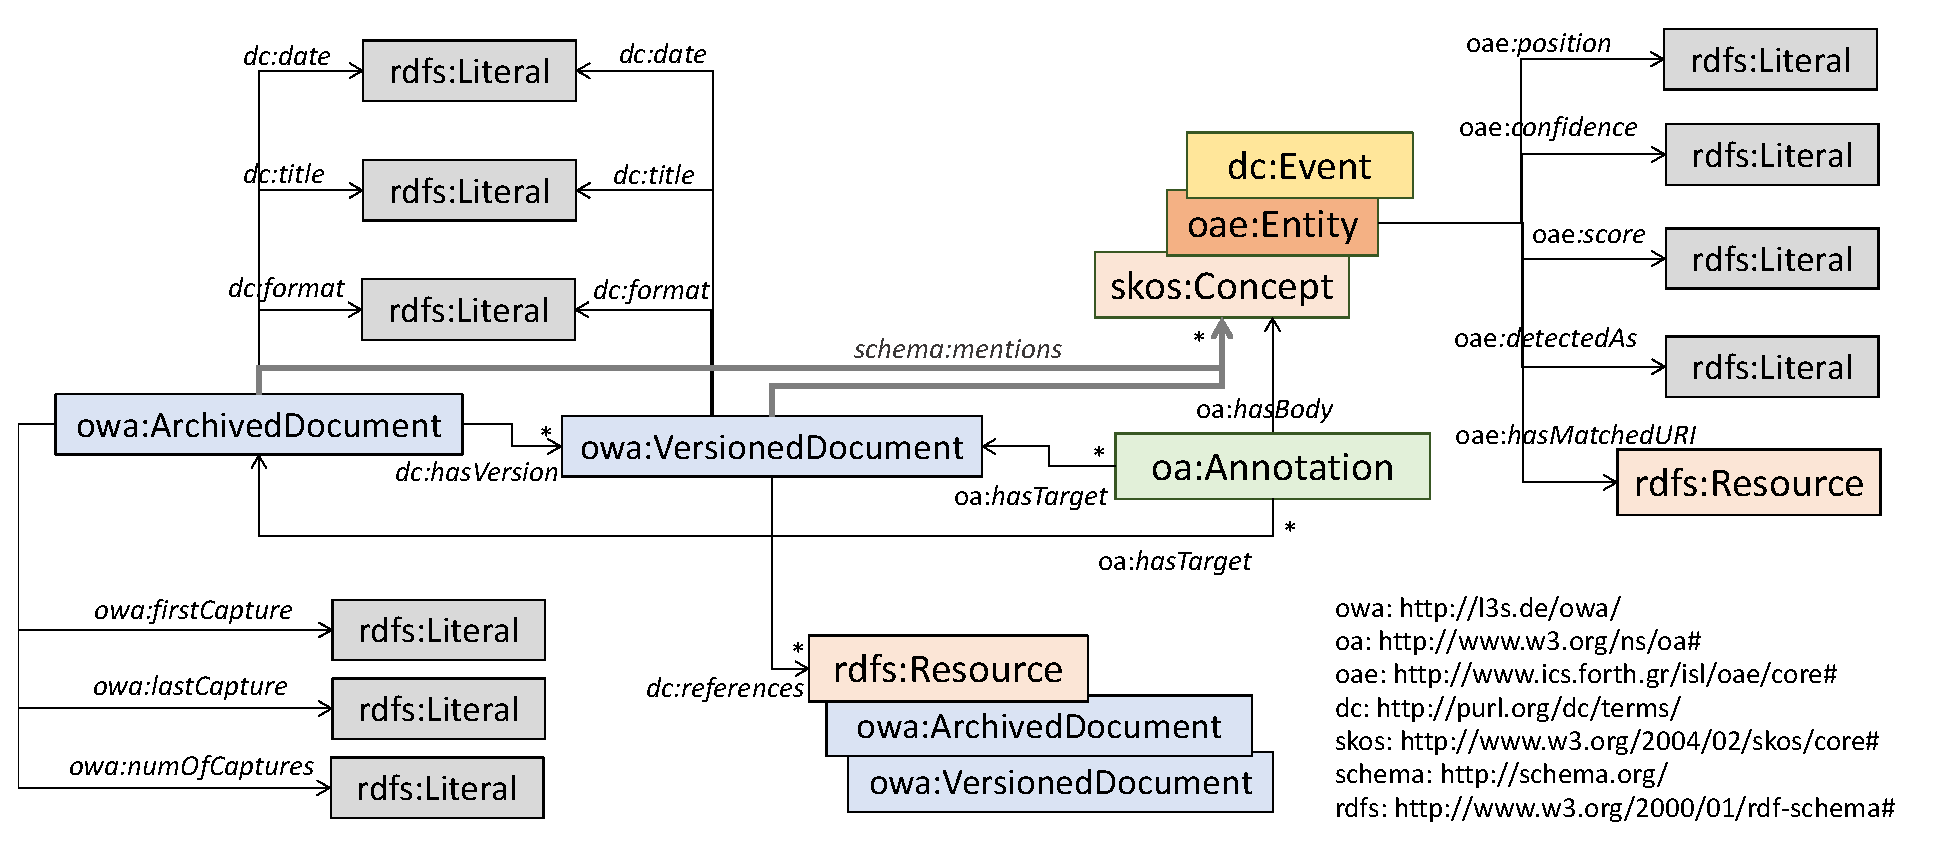
\includegraphics[width=\dimexpr\textwidth-2\fboxsep-2\fboxrule\relax]{figures/owa.eps}}
\caption{The {\em Open Web Archive} data model.}
\label{fig:owa}
\end{figure}

\begin{figure}[H]
\centering
\fbox{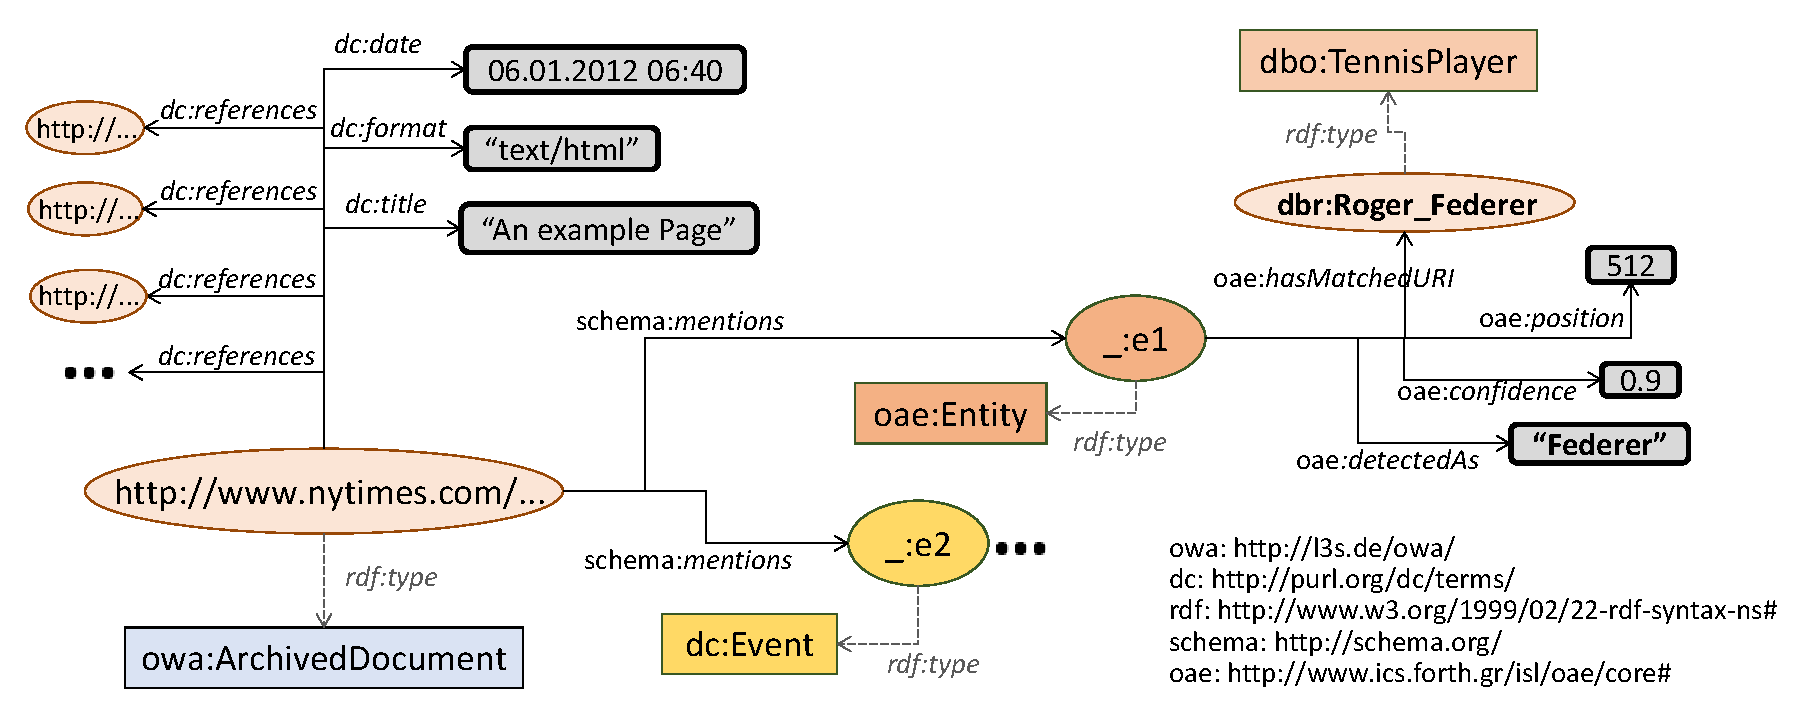
\includegraphics[width=\dimexpr\textwidth-2\fboxsep-2\fboxrule\relax]{figures/owa_inst_nonvers.eps}}
\caption{Describing an archived article (non-versioned) using the {\em Open Web Archive} data model.}
\label{fig:owa_instNonVers}
\end{figure}

Figure \ref{fig:owa_instNonVers} depicts an example of an archived non-versioned article.
Some of its metadata values (date, format, title),
its references to other web pages, and its annotations are visible.
We notice that the entity name \q{Federer} was identified
in that document.
It is also visible that the entity has been linked with the DBpedia resource
corresponding to the tennis player {\em Roger Federer}.
By accessing DBpedia, we can now retrieve more information about this entity
like its birth date, an image, a description in a specific language, etc.
Description of versioned pages using {\em Open Web Archive}
data model is not mentioned in this paper since our
work is mainly focussed on ranking on non-versioned pages.
Details of the construction process of Semantic Layers
have also not been included.
Interested readers should refer to our previous work\cite{fafalios2017SemLayer}
for a more detailed description of this model.

\comment{====
\vspace{0.5mm} \noindent
{\bf Extensibility and Update.}
The proposed model is highly extensible.
For instance, we can
exploit the VoID Vocabulary \cite{alexander2011describing}
and express dataset-related information like
statistics (number of triples, number of entities, etc.),
creation or last modification date,
the subject of the dataset,
collection from which the dataset was derived, etc.
Likewise, one may exploit the PROV data model \cite{moreau2013prov}
and store provenance-related information
(e.g., which tool was used for crawling the documents or for annotating them,
what organizations or people were involved in the crawling or annotation process,
etc.).
In addition, since the contents of the archived documents never change,
we can easily update a semantic layer by just
adding triples in the RDF repository,
e.g., for describing more metadata about the archived documents
or for including new versions.
=====}

\subsection{Related Work (DRAFT)}
\label{rw}

\subsubsection{Ranking of Archived Documents}
\label{arc_doc_ranking}
We mention some of the recent works in the
field of ranking of Archived Documents
using full content based search
or extraction of metadata.

Tempas \cite{holzmann2016tempas}
is a keyword-based search system that exploits a social bookmarking service for
temporally searching a web archive by indexing tags and time.
It allows temporal selections
for search terms, ranks documents based on their
popularity and also provides query recommendations.

Singh et al.\cite{singh2016history}
introduce the notion of {\em Historical Query Intents}
and model it as a search result diversification task
which intends to present the most relevant results (for free text queries) from a
topic-temporal space.
For retrieving and ranking historical documents (e.g., news articles),
the authors propose a novel retrieval algorithm, called HistDiv,
which jointly considers the aspect and time dimensions.

Expedition \cite{singh2016expedition} is a time-aware
search system for scholars.
It allows users to search articles in a news
collection by entering free-text queries and choosing
from four retrieval models:
Temporal Relevance,
Temporal Diversity,
Topical Diversity, and
Historical Diversity.
\comment{====
The results are presented in a
newspaper-style interface, while entity filters
allows users refine the results.
====}

\comment{=====
Excluded as Sindice deals with
RDF Documents in general and
not archived documents.

Sindice\cite{tummarello2007sindice} acts as a locator
service for RDF resources and
returns pointers to the remote data sources.
The ranking is metadata based and
the service ranks the results obtained
after index retrieval on query time
based upon a resource's hostname, external rank
and relevance.
====}

\noindent \textbf{Difference of our approach.} Our approach
provides ranking using structured queries rather than
keyword-based queries.
To provide ranking, we do not access
the content of the articles rather a
layer composed of RDF triples which
contains metadata, links and entities
extracted from the articles.

\subsubsection*{Ranking in Knowledge Graphs}
\label{graph_ranking}

Most of the Ranking Approaches on Knowledge Graphs
are adaptations
of the existing approaches for unstructured data.

Dali et. al.\cite{dali2012query} propose a query
independent Learning to Rank(LTR) approach
for RDF entity search. They use RDF graph extracted features,
search engine based features
and centrality-based features and compare them to target features.
Latifi and Nematbaksh\cite{latifi2014query} also use
the same approach
but suggest the use of Information Content(IC) feature
to reduce ranking time of the system.

OntologyRank algorithm by Ding et al. introduced
in \cite{ding2004swoogle} and mentioned
further in \cite{ding2005finding}
finds use in the Semantic web search engine \emph{Swoogle}.
It identifies Semantic Web Ontologies(SWOs) in Semantic Web
Documents(SWDs) and further ranks terms in an Ontology based on their popularity.
AKTiveRank\cite{alani2006ranking} by Alani et. al.
is another ontology ranking approach which relies
on their importance to a given query
and uses the semantic web search engine
\emph{Swoogle}\cite{ding2005finding} to get a list
of ontologies that need to be ranked.
SemRank\cite{anyanwu2005semrank} designed by
Anwanyu et. al. ranks relationships in SWDs.

Regarding PageRank based approaches, PopRank\cite{nie2005object} 
assigns weights to links among Web Objects
depending on the relationship types between objects.
This system extracts a subset of the graph
based on domain and then assigns link weights
to the subgraph using expert generated Ranking Lists.
Harth et. al.\cite{harth2009using} perform ranking 
by assigning weights to all links in the graphs
based on authority or provenance of data source
and calculating PageRank for the whole
graph even before the query is entered.
This approach is in complete contrast
to ReConRank\cite{hogan2006reconrank}, an
algorithm that performs dynamic ranking only
analysing the result data that matches the user query and 
which considers the ratio of all the links received as
in-links in order to reduce the number of iterations.
RareRank\cite{wei2009semantic} is another 
algorithm where the random component
in the PageRank model is replaced by
a more deterministic component based on
the domain of search in order to reduce randomness in a graph.
DBPediaRanker\cite{mirizzi2010ranking} 
first dereferences and explores all nodes in the
DBPedia graph belonging to the same
domain given a query. Then by checking whether
a strong relation exists between two resources,
it creates a contextualized weighted graph.
YAGO-NAGA introduced in Kasneci et. al.\cite{kasneci2008naga}
and extended to include keyword based search in
Elbassouni et. al.\cite{elbassuoni2009language} is
a semantic search system based on Language Model that
performs ranking based on the notions of Informativeness,
Compactness and Confidence.
DING\cite{delbru2010hierarchical} 
calculates rank in three steps:
first the global dataset rank,
then the entity rank and finally the global ranking
which is a combination of the of both the global
dataset rank and the entity rank.
Fafalios and Tzitzikas\cite{fafalios2014post} integrate
classical Web with the LOD Web using PageRank like algorithm 
to provide users with semantic context 
to help them save
time in exploratory search scenarios.
 
Considering link-based approaches other than
PageRank adaptations, 
NOC-ORDER\cite{graves2008method} introduced by
Graves et. al. is an adaptation of \emph{All-Pairs Shortest Path}
algorithm that ranks nodes in an RDF graph
based on centrality feature.

\comment{====
Older Version(use in case more space available and 
approaches need to be described in greater detail.)

Dali et. al.\cite{dali2012query} propose a query
independent Learning to Rank(LTR) approach
for RDF entity search. They use RDF graph extracted features,
search engine based features
and centrality-based features and compare them to target features.
To obtain the ground truth for the target
features they use human relevance judgements.

Latifi and Nematbaksh\cite{latifi2014query} use
the same approach as that proposed
by Dali et. al.\cite{dali2012query}
but suggest the use of the Information Content(IC) feature
to reduce ranking time of the system.

SemRank\cite{anyanwu2005semrank} designed by
Anwanyu et. al. ranks relationships instead of entities.
The final ranking is calculated based on the predictability
or gain of information of
a semantic association, the degree of similarity
of a keyword or property occurring in a semantic association
and the amount of differences between the properties
in the original schema and the properties that compose a path.

OntologyRank algorithm by Ding et al. introduced
in \cite{ding2004swoogle} and mentioned
further in \cite{ding2005finding}
finds use in the Semantic web search engine \emph{Swoogle}.
It identifies Semantic Web Ontologies(SWOs) in Semantic Web
Documents(SWDs) and further ranks terms in an Ontology based on their popularity.

PopRank\cite{nie2005object} is a variation of PageRank
that assigns weights to links among Web Objects
depending on the relationship types between objects.
This system extracts a subset of the graph
based on domain and then assigns link weights
to the subgraph using Ranking Lists made by domain experts.

ReConRank\cite{hogan2006reconrank} is a PageRank
based algorithm that performs dynamic ranking and only
analyses the result data that matches the user query.
It considers the ratio of all the links received as
in-links in order to reduce the number of iterations
and allows users to fine tune the weights according to their choice.
It goodness relies on the relationships between resources
and their provenance and faces challenges
like extraction of topical graph and increase
in query time due to dynamic ranking.

AKTiveRank\cite{alani2006ranking} by Alani et. al.
is another ontology ranking approach which relies
on their importance to a given query
and uses the semantic web search engine
\emph{Swoogle}\cite{ding2005finding} to get a list
of ontologies that need to be ranked.

YAGO-NAGA introduced in Kasneci et. al.\cite{kasneci2008naga}
and extended to include keyword based search in
Elbassouni et. al.\cite{elbassuoni2009language} is
a semantic search system based on Language Model that
performs ranking based on the notions of Informativeness,
Compactness and Confidence.
The computation is done through a PageRank
like algorithm and
makes use of the provenance of information.

Harth et. al.\cite{harth2009using} use a variation
of the PageRank algorithm for ranking in which
they assign weights to all links in the graphs
based on authority or provenance of data source
and calculate PageRank for the whole
graph even before the query is entered.
This approach is in complete contrast
to ReConRank\cite{hogan2006reconrank} approach.

RareRank\cite{wei2009semantic} is another PageRank
like algorithm where the random component
in the PageRank model is replaced by
a more deterministic component based on
the domain of search in order to reduce randomness in a graph.

DBPediaRanker\cite{mirizzi2010ranking} tries to
first dereference and explore all nodes in the
DBPedia graph belonging to the same
domain given a query. Then by checking whether
a strong relation exists between two resources,
it creates a contextualized weighted graph
with the weights of links between two resources
based on the similarity between nodes.

DING\cite{delbru2010hierarchical} is another adaptation
of the PageRank algorithm which calculates rank in three steps.
First it calculates the global dataset rank,
then the entity rank and finally the global ranking
which is a combination of the of both the global
dataset rank and the entity rank.

NOC-ORDER\cite{graves2008method} introduced by
Graves et. al. ranks nodes in an RDF graph
based on centrality feature.
The algorithm is an adaptation of \emph{All-Pairs Shortest Path}
algorithm for RDF graph and tries to
rank nodes based on the connectedness
and distance of each node to the other nodes.

Fafalios and Tzitzikas\cite{fafalios2014post} integrate
classical Web with the Web of Linked Data to provide
users with semantic context and thus help users save
time in exploratory search scenarios.
For the top-100 results from BING search engine
for keyword search query, the system detects the entities in the snippets of the
results. For the top-k entities derived from a PageRank like algorithm,
the system then using the information available
on the LOD Cloud tries
to show the user how the top detected entities are related.

====}

\noindent \textbf{Difference of our approach.} Our work ranks documents
rather than entities, relationships \cite{anyanwu2005semrank}
or ontologies (\cite{ding2004swoogle}, \cite{ding2005finding}
and \cite{alani2006ranking}).
Unlike \cite{dali2012query} and
\cite{latifi2014query}, our approach does not require any training data.
It does not use any kind of link analysis like in \cite{hogan2006reconrank}, \cite{kasneci2008naga},
\cite{elbassuoni2009language}, \cite{harth2009using}, \cite{wei2009semantic}, \cite{delbru2010hierarchical}
and \cite{graves2008method}.
Further, its not domain specific like \cite{anyanwu2005semrank} and \cite{nie2005object},
doesn't rely on provenance of data sources as in \cite{kasneci2008naga}, \cite{elbassuoni2009language} and \cite{harth2009using} and
produces the ranking at query-execution time unlike \cite{hogan2006reconrank}.

\subsubsection{Ranking Documents in Knowledge Graphs}
\label{sec:graph_doc_ranking}
Little work has been done on ranking documents
in knowledge graphs.

Swoogle, the Semantic web search engine, uses
the OntologyRank algorithm \cite{ding2004swoogle}, \cite{ding2005finding}
as mentioned in the previous sub-section and operates at the document level
as well as the term and RDF graph level. It calculates relevance
of Semantic Web Documents based on whether a document imports,
uses, extends definition of the other document's terms or
makes assertions about the individuals defined by the other document.

\noindent \textbf{Difference of our approach.} Our approach does
not judge relevance of documents based on the relationships
between the documents, because our problem
is to rank a set of relevant documents rather than rank on the relevance
of documents. To the best of our knowledge, we are the very first authors
to perform such ranking using Semantic Models/Layers.